\input{LaTeX/econtexRoot}\input{\econtexRoot/LaTeX/econtexPaths}
\documentclass{beamer}
\usepackage{etoolbox}
\usepackage{comment}
\usepackage{graphicx}
% \usepackage{dtklogos}
\usepackage{dsfont}
\usepackage{amsmath,amssymb}
\usepackage{\econtexShortcuts}
\usepackage[english]{babel}
\usepackage[svgnames,hyperref]{}
\usepackage{empheq}
\usepackage[many]{tcolorbox}
\usepackage{remreset}
\usepackage{tikz} 
\usetikzlibrary{tikzmark,fit,shapes.geometric}
\usetikzlibrary{tikzmark,calc,arrows,shapes,decorations.pathreplacing}
\tikzset{every picture/.style={remember picture}}
\usepackage{cancel}
\usepackage{booktabs,natbib}
\setbeamercovered{invisible}

\usepackage{dcolumn}

\tcbset{highlight math style={enhanced,
    colframe=red!60!black,colback=yellow!50!white,arc=4pt,boxrule=1pt,
  }}

\definecolor{darkblue}{rgb}{0.055,0.094,0.7}
\definecolor{darkred}{rgb}{0.6,0,0}

\hypersetup{colorlinks=true,           % put a box around links
  linkbordercolor = {1 0 0}, % the box will be red
  pdfborder = {1 0 0},       % 
  % bookmarks=true,            % PDF will contain an index on the RHS
  urlcolor=darkred,
  citecolor=darkblue,
  linkcolor=darkred
}



\makeatletter
\@removefromreset{subsection}{section}
\patchcmd{\beamer@part}{\setcounter{subsection}{0}}{}{}
\makeatother
\setcounter{subsection}{1}
\setbeamercovered{transparent}
\setbeamertemplate{navigation symbols}{}%remove navigation symbols
\begin{comment}
  \setbeamertemplate{footline}
  {
    \hbox{\begin{beamercolorbox}[wd=1\paperwidth,ht=2.25ex,dp=1ex,right]{framenumber}%
        \usebeamerfont{framenumber}\insertframenumber{} \hspace*{2ex}
      \end{beamercolorbox}}%
    \vskip0pt%
  }
\end{comment}


\mode<presentation>{}

\title[Modeling the Consumption Response to the CARES Act]{Modeling the Consumption Response\\ to the CARES Act}
\author[]{Christopher D. Carroll \and Edmund Crawley \and Jiri Slacalek \and Matthew N. White}
\date[05/20/2020]{May 20, 2020 \vspace{0.5cm} \\ Presentation at JHU Modeling and Policy Town Hall \\  \vspace{1cm} \footnotesize Viewpoints and conclusions stated in this paper are the responsibility of the authors alone and do not necessarily reflect the viewpoints of the Federal Reserve Board or the ECB.}
\usetheme{Frankfurt}

\setbeamertemplate{navigation symbols}{}
\makeatletter
\setbeamertemplate{footline}
{%
  \hbox{\begin{beamercolorbox}[wd=1\paperwidth,ht=2.25ex,dp=1ex,right]{framenumber}%
      \usebeamerfont{framenumber}\insertframenumber{} \hspace*{2ex}
    \end{beamercolorbox}}%
  \vskip0pt%
  \pgfuseshading{beamer@barshade}%
  \ifbeamer@sb@subsection%
  \vskip-9.75ex%
  \else%
  \vskip-7ex%
  \fi%
  \begin{beamercolorbox}[ignorebg,ht=2.25ex,dp=3.75ex]{section in head/foot}
    \insertnavigation{\paperwidth}
  \end{beamercolorbox}%
  \ifbeamer@sb@subsection%
  \begin{beamercolorbox}[ignorebg,ht=2.125ex,dp=1.125ex,%
    leftskip=.3cm,rightskip=.3cm plus1fil]{subsection in head/foot}
    \usebeamerfont{subsection in head/foot}\insertsubsectionhead \insertframenumber{} \hspace*{2ex}
  \end{beamercolorbox}%
  \fi%
}%
\setbeamertemplate{headline}{%
}
\makeatother
\begin{document}
\setbeamertemplate{caption}{\raggedright\insertcaption\par}
\newcolumntype{d}[1]{D{.}{.}{#1}}
% circled draws a circle around a number
\newcommand*\circled[1]{\tikz[baseline=(char.base)]{
    \node[shape=circle,draw,inner sep=2pt] (char) {#1};}}

\begin{frame}
  \titlepage
\end{frame}


\begin{frame}\frametitle{About this Project}
  Modeling Topic: Timing and Magnitude of Consumer Spending
  
  \medskip
  Quick Takeaways:
  \begin{itemize}
  \item Big negative effect on spending during lockdown
  \item Consumer ``stimulus'' part of CARES act was large
  \end{itemize}

  $\Rightarrow$ when lockdown ends, pretty substantial cash-on-hand
  \begin{itemize}
  \item Detailed distributional data: history/models
    \begin{itemize}
    \item  $\Rightarrow$ lots of spending
    \end{itemize}
  \end{itemize}

  Gaps:

  \begin{itemize}
  \item Computational (Programming) Resources
  \item Integration With Epidemiological Model Inputs
  \end{itemize}

  \medskip
  
  Interesting Finding:
  \begin{itemize}
  \item The UI Component Is Big Enough -- While It Lasts
  \end{itemize}
\end{frame}
\begin{frame}{Links}
  \begin{footnotesize}
    \parbox{\textwidth}{
      \begin{center}
        \begin{tabbing}
          \= \href{https://econ-ark.github.io/Pandemic}{econ-ark.github.io/Pandemic}     \= \textit{~~~~HTML version of paper}                                         \\
          \> \href{https://econ-ark.org/pandemicdashboard}{Interactive-Jupyter-Notebook} \> \textit{~~~~Allows user to modify some assumptions}                      \\
          \> \href{https://github.com/econ-ark/Pandemic}{github.com/econ-ark/Pandemic}   \> \textit{~~~~Full codebase; explore all assumptions} \\
          \> \href{https://github.com/econ-ark/Pandemic/blob/master/LaTeX/ConsumptionResponse.pdf}{~~LaTeX subdirectory of $\uparrow$}     \> \textit{~~~~PDF version of paper}                                         \\
          \> \href{https://github.com/econ-ark/Pandemic/blob/master/LaTeX/ConsumptionResponse-Slides.pdf}{~~LaTeX subdirectory of $\uparrow$}     \> \textit{~~~~Presentation slides}                                         \\
        \end{tabbing}
      \end{center}
    }
  \end{footnotesize}

\end{frame}
\addtocounter{framenumber}{-1}
\section{Model}
\setbeamercovered{invisible}
\frame{
  \frametitle{The CARES Act}
  The CARES Act directly impacts household balance sheets:
  \begin{itemize}
  \item \$1,200 to every adult (means tested)
  \item \$600 per week \textit{additional} unemployment benefits, for up to 13 weeks (\$7,800)
  \end{itemize}
  Compared to 10 years ago, we now have good models of how household consumption responds\\
  \bigskip
  Contribution of paper:
  \begin{itemize}
  \item How is this time different?
  \item What does a carefully calibrated consumption model say?
  \end{itemize}
}
\frame{
  \frametitle{What's Old - Baseline Model}
  Rich stochastic lifecycle model made up of high school dropouts, high school graduates and college graduates, matching:
  \begin{itemize}
  \item Their income profiles (trends and uncertainty)
  \item Liquid wealth	distribution
    \begin{itemize}
    \item matched using patience heterogeneity
    \end{itemize}
  \end{itemize}
  
  $\Rightarrow$ Annual Marginal Propensity to Consume (MPC) $\approx$ 0.5\\
  \bigskip
  Matches \textit{both} micro and macro phenomena
  \begin{itemize}
  \item \cite{psjmMPC2008}
  \item \cite{fhnMPC}
  \end{itemize}
}
\frame{
  \frametitle{What's New: (1) `Deep' Unemployment}
  Want to experiment with different expectations (and realities) about the length of pandemic-related unemployment.\\
  \medskip
  Two types of unemployed:
  \begin{itemize}
  \item[1] `Normal' Unemployed: 2/3 probability of finding a job each quarter - expected unemployment duration 1.5 quarters
  \item[2] `Deep' Unemployed: 1/3 probability of returning to `normal' unemployed state each quarter - expected unemployment duration 4.5 quarters
  \end{itemize}
}
\frame{
  \frametitle{What's New: (2) `Lockdown' Consumption}
  $C$ during lockdown is restricted:
  \begin{itemize}
  \item Many types of $C$ less desirable, or illegal
  \item Calibration: 11 percent $C$ reduction (travel, restaurants, etc)
  \item Captured by reduction in the marginal utility of $C$
  \end{itemize}

  $\Rightarrow$ Households defer some of their spending into the future
}
\frame{
  \frametitle{Calibrating the Pandemic}
  Two scenarios:
  \begin{itemize}
  \item Short-Lived: `Lockdown' lasts two quarters on average
    \begin{itemize}
    \item unemployment 15\%
    \item One-third is `deep unemployment'
    \end{itemize}
  \item Long, Deep: The `lockdown' lasts four quarters on average
    \begin{itemize}
    \item unemployment 22\%
    \item Mostly deep unemployment
    \end{itemize}
  \end{itemize}
  \medskip
%  BUT these assumptions are highly contested and rapidly changing with data\\
  We invite you to make your own assumptions:\\
  \hypertarget{links}{}
  \begin{small}
    \parbox{\textwidth}{
      \begin{center}
        \begin{tabbing}
          \= \href{https://econ-ark.org/pandemicdashboard}{Interactive-Jupyter-Notebook} \= \textit{~~~~Allows user to modify some assumptions}                      \\
          \> \href{https://github.com/econ-ark/Pandemic}{github.com/econ-ark/Pandemic}   \> \textit{~~~~Full codebase} \\
        \end{tabbing}
      \end{center}
    }
  \end{small}
}
\frame{
  \frametitle{Unemployment skews young, unskilled and low income}
  \begin{figure}
    \centering
    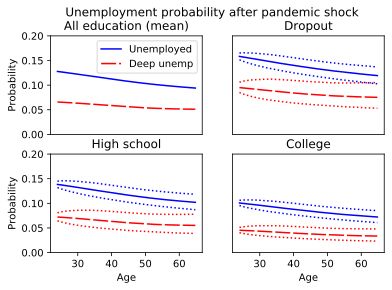
\includegraphics[width=0.9\textwidth]{\econtexRoot/Figures/UnempProbByDemogBasic}
  \end{figure}
}
\frame{
  \frametitle{Aggregate Labor and Transfer Income}
  \begin{figure}
    \centering
    \includegraphics[width=0.9\textwidth]{\econtexRoot/Figures/AggLT}
  \end{figure}
  {\footnotesize Assumes: Stimulus check delayed one qtr; 25 percent spend before check}
}
\section{Results}
\frame{
  \frametitle{Aggregate Consumption Response}
  \begin{figure}
    \centering
    \includegraphics[width=0.9\textwidth]{\econtexRoot/Figures/AggConResp_examples}
  \end{figure}
}
\frame{
  \frametitle{Consumption Response Decomposition}
  \begin{figure}
    \centering
    \includegraphics[width=0.9\textwidth]{\econtexRoot/Figures/Decomposition}
  \end{figure}
}
\frame{
  \frametitle{Consumption Response By Employment Type}
  \begin{tikzpicture}
    \node (img1) {\includegraphics[width=0.9\textwidth,clip]{\econtexRoot/Figures/ConRespByEmpStateNoStim}};
    \pause
    \node (img2) {\includegraphics[width=0.9\textwidth,clip]{\econtexRoot/Figures/ConRespByEmpStateWStim}};
    \onslide<1->
  \end{tikzpicture}
}
\frame{
  \frametitle{Consumption Response By Employment Type}
  \begin{figure}
    \centering
    \includegraphics[width=0.9\textwidth]{\econtexRoot/Figures/ConDeltaByEmpState}
  \end{figure}
}
\frame{
  \frametitle{Is Targeting Useful In The Aggregate?}
  \begin{figure}
    \centering
    \includegraphics[width=0.7\textwidth]{\econtexRoot/Figures/EffectTargeting}
  \end{figure}
  \begin{itemize}
  \item Deep unemployed have lower MPCs
  \item UE benefits are generous - average MPC lower than marginal
  \end{itemize}
}
\frame{
  \frametitle{Deep, Long Pandemic: Income}
  \begin{figure}
    \centering
    \includegraphics[width=0.9\textwidth]{\econtexRoot/Figures/AggLT_long_pandemic}
  \end{figure}
}
\frame{
  \frametitle{Deep, Long Pandemic: Consumption}
  \begin{figure}
    \centering
    \includegraphics[width=0.9\textwidth]{\econtexRoot/Figures/DeepPandemic}
  \end{figure}
}
\frame{
  \frametitle{Conclusions}
  Short-lived lockdown: CARES Act sufficient for swift $C$ recovery\\
  \bigskip
  Long, deep lockdown: Further action to prevent big $C$ drop\\
  \bigskip
  \medskip
  
  Check out the dashboard:

  \centerline{\url{https://econ-ark.org/pandemicdashboard}}
}

\bibliographystyle{\econtexBibStyle}
\newsavebox\mytempbib
\savebox\mytempbib{\parbox{\textwidth}{\bibliography{\econtexRoot/LaTeX/ConsumptionResponse,\econtexRoot/LaTeX/ConsumptionResponse-Add}}}


\end{document}


% Local Variables:
% TeX-PDF-mode: t
% TeX-command-extra-options: "-output-directory=LaTeX"
% End:
